\begin{pastexam}[label={px:df3-113-ds-05}]{地方三等資訊處理 113 年 第五題}
（申論；15 分）

下面的矩陣 $M$ 是表示一個無向圖 $G$=($V$, $E$)的相鄰矩陣（Adjacency Matrix），$V$ 與 $E$ 分別為節點與邊的集合：
\begin{center}
\begin{tabular}{|c|c|c|c|c|c|c|c|}
\hline
 & $\bm{a}$ & $\bm{b}$ & $\bm{c}$ & $\bm{d}$ & $\bm{e}$ & $\bm{f}$ & $\bm{g}$ \\ \hline
$\bm{a}$ & 0 & 1 & 0 & 1 & 1 & 1 & 0 \\ \hline
$\bm{b}$ & 1 & 0 & 1 & 0 & 1 & 1 & 0 \\ \hline
$\bm{c}$ & 0 & 1 & 0 & 0 & 0 & 1 & 1 \\ \hline
$\bm{d}$ & 1 & 0 & 0 & 0 & 0 & 0 & 1 \\ \hline
$\bm{e}$ & 1 & 1 & 0 & 0 & 0 & 0 & 0 \\ \hline
$\bm{f}$ & 1 & 1 & 1 & 0 & 0 & 0 & 1 \\ \hline
$\bm{g}$ & 0 & 0 & 1 & 1 & 0 & 1 & 0 \\ \hline
\end{tabular}
\end{center}
\begin{enumerate}[leftmargin=2.6em, labelsep=0.4em]
\item[㈠] 請畫出此無向圖 $G$。（10 分）
\item[㈡] 若以字母順序為考量對 $G$ 進行廣度優先搜尋（Breadth-First Search, BFS），因此將由節點 $a$ 開始，請繪出
尋訪完後所產生的 BF 樹（Breadth-First (BF) Tree）。（5 分）
\end{enumerate}
\end{pastexam}

\begin{pastsoln}
\textbf{㈠} 矩陣是對稱的（$M[u][v] = M[v][u]$），對角線全是 $0$，表示沒有自迴圈，符合無向圖。 讀上三角形
（$u < v$ 且 $M[u][v] = 1$）得到邊：
\[
E = \{ab, ad, ae, af, bc, be, bf, cf, cg, dg, fg\},
\]
共 $11$ 條（每列 $1$ 的個數就是度數：$a{:}4$、$b{:}4$、$c{:}3$、$d{:}2$、$e{:}2$、$f{:}4$、$g{:}3$，總和 $22 = 2 \times 11$）。
\begin{center}
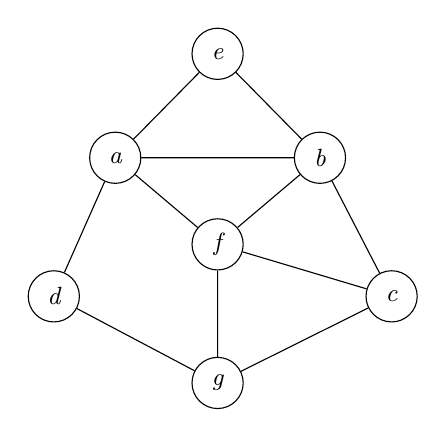
\begin{tikzpicture}[x=1.3cm,y=1.1cm,v/.style={circle,draw,inner sep=0pt,minimum size=6.5mm,font=\small\itshape}]
\node[v] (e) at (1,1.2) {e};
\node[v] (a) at (0,0) {a};
\node[v] (b) at (2,0) {b};
\node[v] (f) at (1,-1) {f};
\node[v] (d) at (-0.6,-1.6) {d};
\node[v] (c) at (2.7,-1.6) {c};
\node[v] (g) at (1,-2.6) {g};
\draw (a)--(b) (a)--(d) (a)--(e) (a)--(f) (b)--(c) (b)--(e) (b)--(f) (c)--(f) (c)--(g) (d)--(g) (f)--(g);
\end{tikzpicture}
\end{center}
（畫法不唯一，只要頂點和邊對得上即可。）

\textbf{㈡} BFS（資結書第~21.3~節）從 $a$ 出發，用佇列；取出一個頂點時，依字母順序看它的鄰居，還沒拜訪過的
就標記、記下父節點、放進佇列。
\begin{center}
\small
\begin{tabular}{clll}
\toprule
取出 & 鄰居（字母順序） & 新發現（父節點） & 佇列（取出後、加入後） \\
\midrule
--- & & $a$（起點） & $a$ \\
$a$ & $b, d, e, f$ & $b, d, e, f$（父 $a$） & $b, d, e, f$ \\
$b$ & $a, c, e, f$ & $c$（父 $b$） & $d, e, f, c$ \\
$d$ & $a, g$ & $g$（父 $d$） & $e, f, c, g$ \\
$e$ & $a, b$ & 無 & $f, c, g$ \\
$f$ & $a, b, c, g$ & 無 & $c, g$ \\
$c$ & $b, f, g$ & 無 & $g$ \\
$g$ & $c, d, f$ & 無 & 空 \\
\bottomrule
\end{tabular}
\end{center}
拜訪順序 $a, b, d, e, f, c, g$。 BF 樹由「父節點 $\to$ 新發現」的邊組成：$ab, ad, ae, af, bc, dg$，共 $6 = 7 - 1$ 條。
\begin{center}
\begin{tikzpicture}[v/.style={circle,draw,inner sep=0pt,minimum size=6.5mm,font=\small\itshape},
  level distance=11mm, level 1/.style={sibling distance=15mm}]
\node[v] {a}
  child {node[v] {b} child {node[v] {c}}}
  child {node[v] {d} child {node[v] {g}}}
  child {node[v] {e}}
  child {node[v] {f}};
\node[font=\small,anchor=west] at (3.2,0) {距離 $0$};
\node[font=\small,anchor=west] at (3.2,-1.1) {距離 $1$};
\node[font=\small,anchor=west] at (3.2,-2.2) {距離 $2$};
\end{tikzpicture}
\end{center}
樹上每個頂點的深度就是它到 $a$ 的最短距離（邊數）：$b, d, e, f$ 是 $1$，$c, g$ 是 $2$。 注意 $c$ 也和 $f$ 相鄰、
$g$ 也和 $c, f$ 相鄰，但依字母順序 $b$ 先被取出，$c$ 由 $b$ 發現；$d$ 比 $f$ 先取出，$g$ 由 $d$ 發現。
\end{pastsoln}
